\section{Execution}
\label{sec:Execution}

The execution will be split up in different segments, so we can focus on the steps necessary to get the absorption spectrum of Rubidium.
During the entire runtime of the experiment everyone in the room needs to wear safety goggles!

\subsection{Setting up the laser}
\label{ssec:exe1}

Assuming the laser has already heaten up and reaches its optimum temperature we need to align the laser first.
For that you need to assemble the diode laser to the optical breadboard.
In its direction of emmitting we put the Rubidum absorption cell and behind it a photodiode detector to register the laserbeam.
Now we need to align the laser, so that its beam goes directly into the cell.
For that the laser is not visible for the human eye we need the IR Card to see its position. 
The orange circle area of the card emitts light if hit with the laserbeam. 
With this method you can locate the laser, although it is invisible.
Put the TV camera in front of the card, so that you can observe the emitted light clearly.
Your setup should look like \autoref{fig:part1}.
\begin{figure}
    \centering
    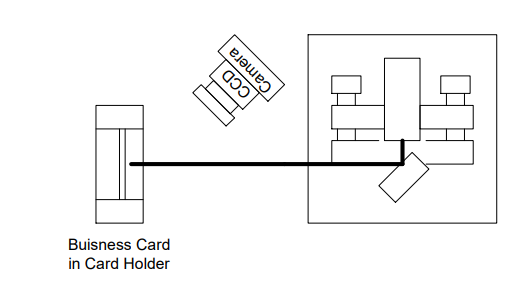
\includegraphics[width=\textwidth]{images/part1.png}
    \caption{Setup for lining up the laser \cite{V60}}
    \label{fig:part1}
\end{figure}
Now we increase the current of the laser, until spreckles are visible on the card. 
The laser is now lasing. 

Something about gain or so.

\subsection{Calibration of the absorption wavelength}
\label{ssec:exe2}
